%
% ---------------------------------------------------------------
% Copyright (C) 2012-2018 Gang Li
% ---------------------------------------------------------------
%
% This work is the default powerdot-tuliplab style test file and may be
% distributed and/or modified under the conditions of the LaTeX Project Public
% License, either version 1.3 of this license or (at your option) any later
% version. The latest version of this license is in
% http://www.latex-project.org/lppl.txt and version 1.3 or later is part of all
% distributions of LaTeX version 2003/12/01 or later.
%
% This work has the LPPL maintenance status "maintained".
%
% This Current Maintainer of this work is Gang Li.
%
%latex slides.tex 
%dvips slides.dvi
%ps2pdf slides.ps
\documentclass[
 size=14pt,
 paper=smartboard,  %a4paper, smartboard, screen
 mode=present, 		%present, handout, print
 display=slides, 	% slidesnotes, notes, slides
 style=tuliplab,  	% TULIP Lab style
 pauseslide,
 fleqn,leqno]{powerdot}

\usepackage{cancel}
\usepackage{caption}
\usepackage{stackengine}
\usepackage{smartdiagram}
\usepackage{attrib}
\usepackage{amssymb}
\usepackage{amsmath} 
\usepackage{amsthm} 
\usepackage{mathtools}
\usepackage{rotating}
\usepackage{graphicx}
\usepackage{boxedminipage}
\usepackage{rotate}
\usepackage{calc}
\usepackage[absolute]{textpos}
\usepackage{psfrag,overpic}
\usepackage{fouriernc}
\usepackage{pstricks,pst-3d,pst-grad,pstricks-add,pst-text,pst-node,pst-tree}
\usepackage{moreverb,epsfig,subfigure}
\usepackage{color}
\usepackage{booktabs}
\usepackage{etex}
\usepackage{breqn}
\usepackage{multirow}
\usepackage{natbib}
\usepackage{bibentry}
\usepackage{gitinfo2}
\usepackage{siunitx}
\usepackage{nicefrac}
\usepackage{media9}
\usepackage{animate}
\usepackage{auto-pst-pdf}
\usepackage{breakurl}
\usepackage{fontawesome}
\usepackage{xcolor}
\usepackage{multicol}



\usepackage{verbatim}
\usepackage[utf8]{inputenc}
\usepackage{dtk-logos}
\usepackage{tikz}
\usepackage{adigraph}
\usepackage{hyperref}
\usepackage{pgfplots}
\usepackage{verbatim}
\usepackage{fontawesome}


\usepackage{todonotes}
\usepackage{animate}
\usepackage{fontawesome}

\usepackage{listings}
\lstset{frameround=fttt,
frame=trBL,
stringstyle=\ttfamily,
backgroundcolor=\color{yellow!20},
basicstyle=\footnotesize\ttfamily}
\lstnewenvironment{code}{
\lstset{frame=single,escapeinside=`',
backgroundcolor=\color{yellow!20},
basicstyle=\footnotesize\ttfamily}
}{}


\usepackage{hyperref}
\hypersetup{ % TODO: PDF meta Data
  pdftitle={Presentation Title},
  pdfauthor={Gang Li},
  pdfpagemode={FullScreen},
  pdfborder={0 0 0}
}


% \usepackage{auto-pst-pdf}
% package to show source code

\definecolor{LightGray}{rgb}{0.9,0.9,0.9}
\newlength{\pixel}\setlength\pixel{0.000714285714\slidewidth}
\setlength{\TPHorizModule}{\slidewidth}
\setlength{\TPVertModule}{\slideheight}
\newcommand\highlight[1]{\fbox{#1}}
\newcommand\icite[1]{{\footnotesize [#1]}}

\newcommand\twotonebox[2]{\fcolorbox{pdcolor2}{pdcolor2}
{#1\vphantom{#2}}\fcolorbox{pdcolor2}{white}{#2\vphantom{#1}}}
\newcommand\twotoneboxo[2]{\fcolorbox{pdcolor2}{pdcolor2}
{#1}\fcolorbox{pdcolor2}{white}{#2}}
\newcommand\vpspace[1]{\vphantom{\vspace{#1}}}
\newcommand\hpspace[1]{\hphantom{\hspace{#1}}}
\newcommand\COMMENT[1]{}

\newcommand\placepos[3]{\hbox to\z@{\kern#1
        \raisebox{-#2}[\z@][\z@]{#3}\hss}\ignorespaces}

\renewcommand{\baselinestretch}{1.2}


\newcommand{\draftnote}[3]{
	\todo[author=#2,color=#1!30,size=\footnotesize]{\textsf{#3}}	}
% TODO: add yourself here:
%
\newcommand{\gangli}[1]{\draftnote{blue}{GLi:}{#1}}
\newcommand{\shaoni}[1]{\draftnote{green}{sn:}{#1}}
\newcommand{\gliMarker}
	{\todo[author=GLi,size=\tiny,inline,color=blue!40]
	{Gang Li has worked up to here.}}
\newcommand{\snMarker}
	{\todo[author=Sn,size=\tiny,inline,color=green!40]
	{Shaoni has worked up to here.}}

%%%%%%%%%%%%%%%%%%%%%%%%%%%%%%%%%%%%%%%%%%%%%%%%%%%%%%%%%%%%%%%%%%%%%%%%
% title
% TODO: Customize to your Own Title, Name, Address
%
\title{Predict future sales}
\author{
Pengcheng Jiang
\\
\\JiLin University
}
\date{\gitCommitterDate}


% Customize the setting of slides
\pdsetup{
% TODO: Customize the left footer, and right footer
rf=\href{http://www.tulip.org.au}{
Last Changed by: \textsc{\gitCommitterName}\ \gitVtagn-\gitAbbrevHash\ (\gitAuthorDate)
},
cf={Predict future sales},
}


\begin{document}

\maketitle

\begin{slide}[toc=,bm=]{Overview}
\tableofcontents[content=currentsection,type=1]
\end{slide}

\section{Problem Definition}

%%==========================================================================================
%%
\begin{slide}[toc=,bm=]{Predict future sales}
  \begin{center}
    \twotonebox{\parbox{.1\textwidth}{given}}{\parbox{.76\textwidth}
    {
      a challenging time-series dataset consisting of daily sales data, kindly provided by one of the largest Russian software firms - 1C Company.
    }}
    \twotonebox{\parbox{.1\textwidth}{target}}{\parbox{.76\textwidth}
    {
      predict total sales for every product and store in the next month
    }}
    \twotonebox{\parbox{.1\textwidth}{evaluate}}{\parbox{.76\textwidth}
    {
      Submissions are evaluated by root mean squared error (RMSE)
    }}
  \end{center}

\end{slide}
%%
%%==========================================================================================

\section{Data Cleaning}


%%==========================================================================================
%%
\begin{slide}[toc=,bm=]{Date}
\begin{table}[h]
  \begin{center}
    \resizebox{\textwidth}{15mm}{
      \begin{tabular}{c| c c c c c c}
      \toprule
      File & \texttt{filed1}  & \texttt{filed2} & \texttt{filed3} & \texttt{filed4} & \texttt{filed5} & \texttt{filed6}\\
      \midrule
      item_categories
      &  item_category_name &  item_category_id \\
      items
      &  item_id &  item_category_id \\
      sales_train
      &  date & date_block_num &  shop_id  & item_id &  item_price &  item_cnt_day \\
      shops
      &  shop_name &  shop_id \\
      test
      &  shop_id &  item_id\\
      \bottomrule
      \end{tabular}
    }
  \end{center}
  \caption{Data Infomation}
\end{table}
\end{slide}
%%
%%==========================================================================================


%%==========================================================================================
%%
\begin{slide}[toc=,bm=]{Data Information}
  \twotonebox{\parbox{.2\textwidth}{sales_train}}{\parbox{.76\textwidth}
  {
    \begin{itemize}
      \item 2935849 rows,6 columns
      \item 21807 items,60 shops
      \item data_type
            \begin{itemize}
              \item data: object
              \item date_block_num: int
              \item shop_id:int
              \item item_id:int
              \item item_price:float
              \item item_cnt_day:float
            \end{itemize}
    \end{itemize}
  }}
\end{slide}
%%
%%==========================================================================================


%%==========================================================================================
%%
\begin{slide}[toc=,bm=]{Data Information}
  \twotonebox{\parbox{.2\textwidth}{test}}{\parbox{.76\textwidth}
  {
    \begin{itemize}
      \item 214200 rows,3 columns
      \item 5100 items,40 shops
      \item data_type
            \begin{itemize}
              \item ID:int
              \item shop_id:int
              \item item_id:int
            \end{itemize}
    \end{itemize}
    From here you can see a lot of stores, goods in training set are not in the test set
  }}
\end{slide}
%%
%%==========================================================================================



%%==========================================================================================
%%
\begin{slide}[toc=,bm=]{Missing Value and Non Value}
  \twotonebox{\parbox{.1\textwidth}{target}}{\parbox{.76\textwidth}
  {
    Find out whether there are empty values or missing values in the data
  }}
  \twotonebox{\parbox{.1\textwidth}{result}}{\parbox{.76\textwidth}
  {
    \begin{itemize}
      \item   missing value:0
      \item   nan value:0
    \end{itemize}
  }}
\end{slide}
%%
%%==========================================================================================

%%==========================================================================================
%%
\begin{slide}[toc=,bm=]{Cartesian product}
  \twotonebox{\parbox{.1\textwidth}{reason}}{\parbox{.76\textwidth}
  {
    The training set contains only the items that the store actually sold that month
  }}
  \twotonebox{\parbox{.1\textwidth}{target}}{\parbox{.76\textwidth}
  {
    for items not sold during the month, you should add them and set them to 0(Find out all the stores and merchandise, and make cartesian product with sales_trainz)
  }}
  
\end{slide}
%%
%%==========================================================================================


%%==========================================================================================
%%
\begin{slide}[toc=,bm=]{Data leakages}
  \twotonebox{\parbox{.1\textwidth}{target}}{\parbox{.76\textwidth}
  {
    delete stores, goods in training set but not in the test set
  }}
  \twotonebox{\parbox{.1\textwidth}{result}}{\parbox{.76\textwidth}
  {
    \begin{itemize}
      \item sales_train:
      \item rows:1224439
      \item items:4716
      \item shops:42
    \end{itemize}
    %\setlength\parindent{2em}sales_train\par
  }}
\end{slide}
%%
%%==========================================================================================


%%==========================================================================================
%%
\begin{slide}[toc=,bm=]{Data duplication}
  \twotonebox{\parbox{.1\textwidth}{target}}{\parbox{.76\textwidth}
  {
    See if duplicate items exist in the dataset
  }}
  \twotonebox{\parbox{.1\textwidth}{result}}{\parbox{.76\textwidth}
  {
    \begin{itemize}
      \item sales_train:6
      \item test:0
    \end{itemize}
  }}
\end{slide}
%%
%%==========================================================================================

%%==========================================================================================
%%
\begin{slide}[toc=,bm=]{Outliers}
  \twotonebox{\parbox{.1\textwidth}{target}}{\parbox{.76\textwidth}
  {
    Calculate the outliers of item_cnt_day and item price
  }}
  \twotonebox{\parbox{.1\textwidth}{result}}{\parbox{.76\textwidth}
  {
    \begin{figure}
      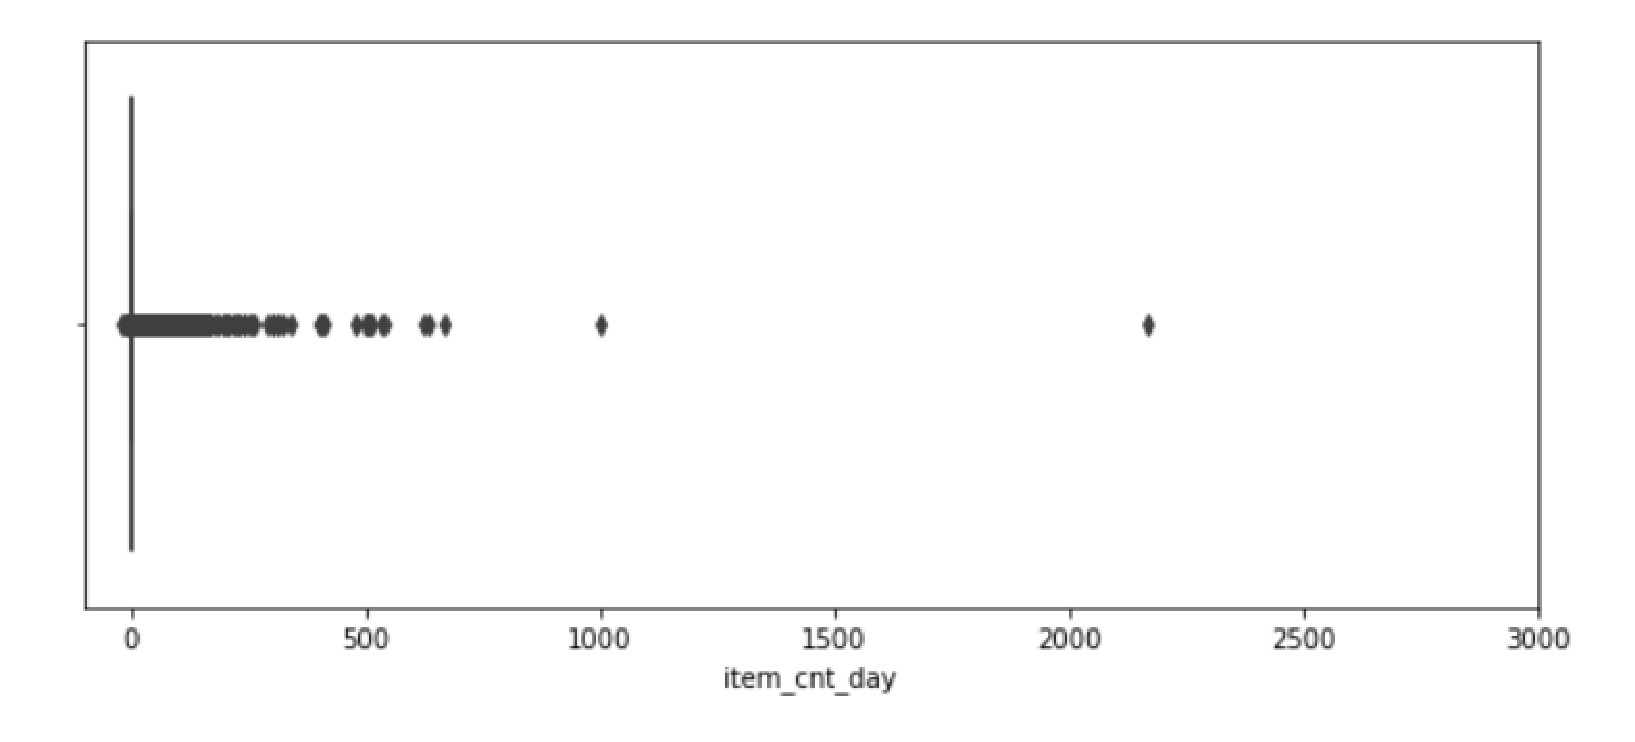
\includegraphics[scale=0.5]{picture/data_7.eps}
    \end{figure}
  }}
\end{slide}
%%
%%==========================================================================================

%%==========================================================================================
%%
\begin{slide}[toc=,bm=]{Outliers}
  \twotonebox{\parbox{.1\textwidth}{result}}{\parbox{.76\textwidth}
  {
    \begin{figure}
      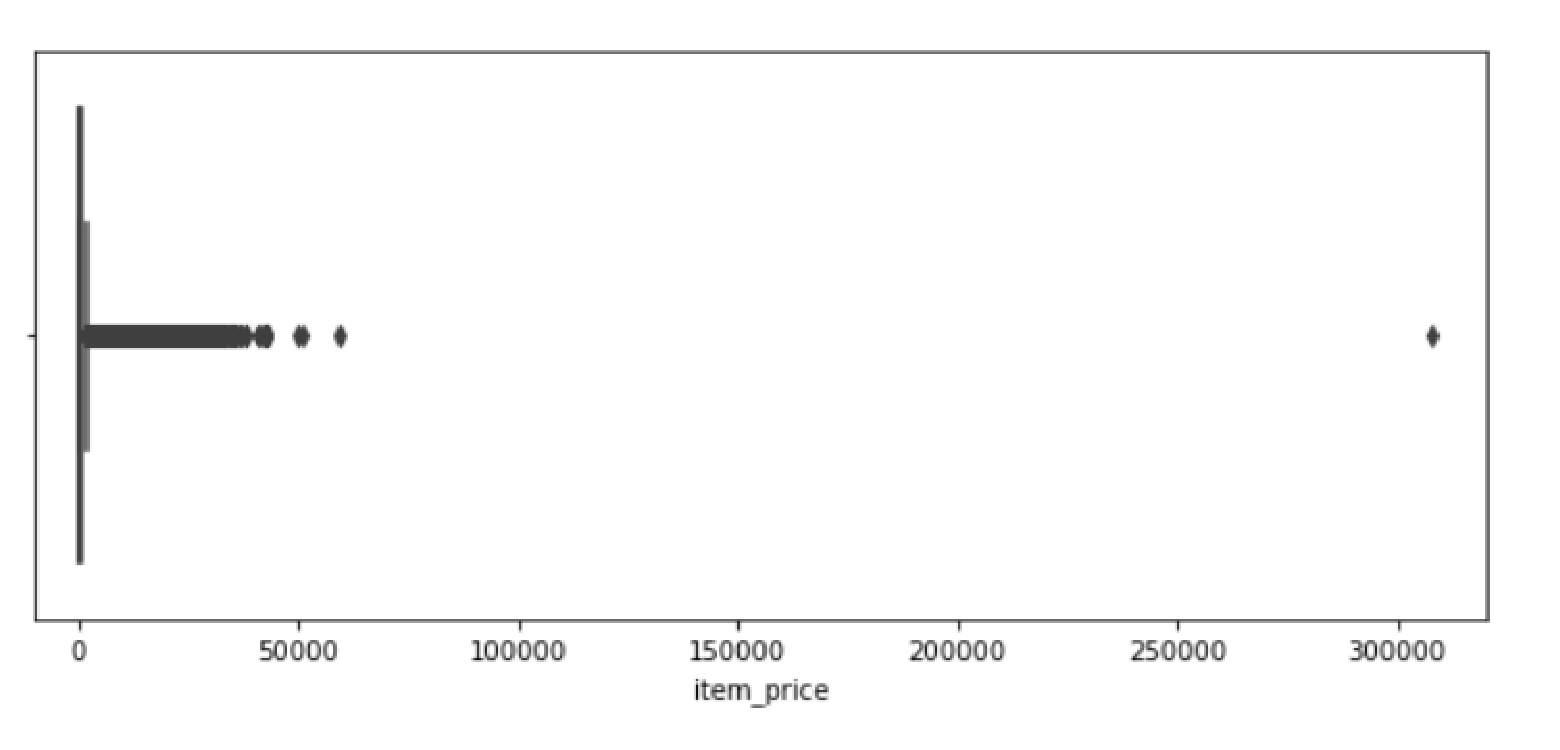
\includegraphics[scale=0.5]{picture/data_8.eps}
    \end{figure}
  }}
\end{slide}
%%
%%==========================================================================================

%%==========================================================================================
%%
\begin{slide}[toc=,bm=]{outdated items and Negative}
  \twotonebox{\parbox{.1\textwidth}{target}}{\parbox{.76\textwidth}
  {
    Analyze how many products have not been sold in the last six consecutive months. How many of these products appear in the test set.
  }}

  \twotonebox{\parbox{.1\textwidth}{result}}{\parbox{.76\textwidth}
  {
    There are 12391 training sets, which have not been sold in the last six months.
    There are 164 test sets, which have not been sold in the last six months
  }}
  \bigskip

\end{slide}
%%
%%==========================================================================================

%%==========================================================================================
%%
\begin{slide}[toc=,bm=]{outdated items and Negative}  
  \twotonebox{\parbox{.1\textwidth}{Negative}}{\parbox{.76\textwidth}
  {
    Change item whose commodity price is negative to median
  }}
\end{slide}
%%
%%==========================================================================================


%%==========================================================================================
%%
\begin{slide}[toc=,bm=]{outdated shops}
  \twotonebox{\parbox{.1\textwidth}{target}}{\parbox{.76\textwidth}
  {
    Analyze how many shops have not been closed
  }}

  \twotonebox{\parbox{.1\textwidth}{result}}{\parbox{.76\textwidth}
  {
    0,  1 , 8, 11 ,13 ,17, 23, 30, 32, 33 ,40 ,43, 54 have been closed
  }}
  \bigskip

\end{slide}
%%
%%==========================================================================================



\section{Data analysis}

%%==========================================================================================
%%
\begin{slide}[toc=,bm=]{Monthly sales of goods}
  \begin{figure}
    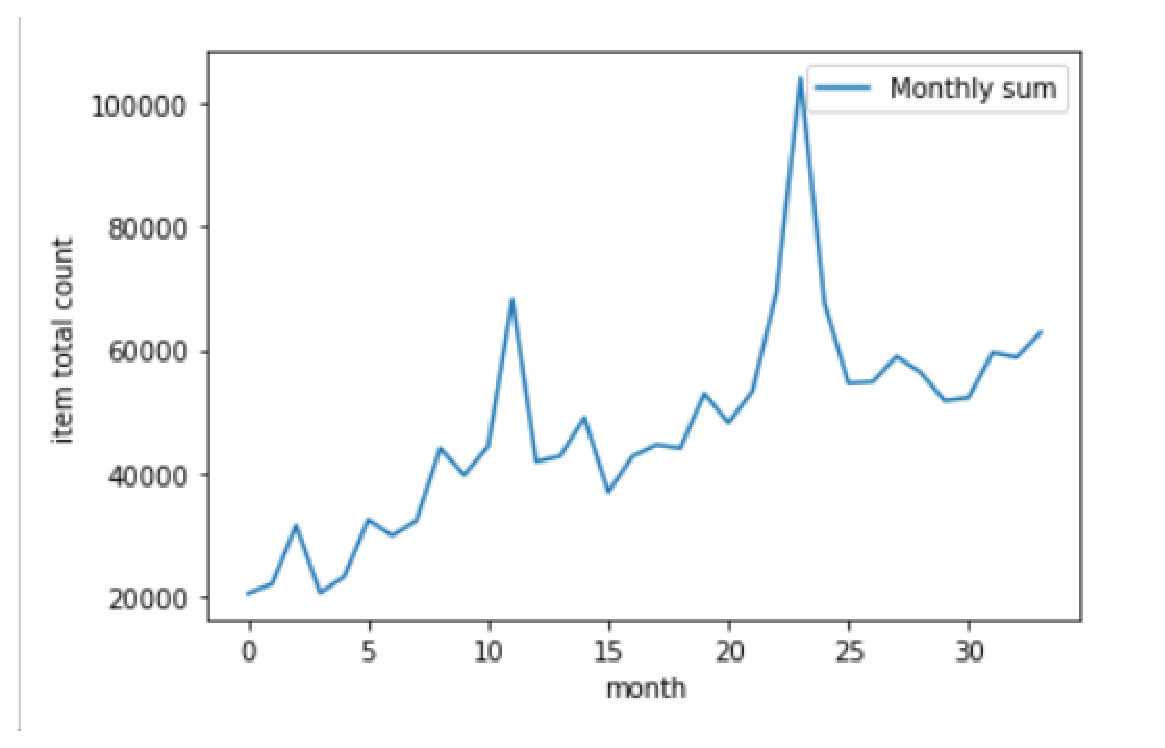
\includegraphics[scale=0.5]{picture/data_20.eps}
  \end{figure}
  \begin{center}
    \textbf{Figure 1}~~month_total_count.\\
  \end{center}
    Explain that the month is related to the sales volume of goods: the sales volume at the end of the year is increasing
\end{slide}
%%
%%==========================================================================================


%%==========================================================================================
%%
\begin{slide}[toc=,bm=]{Shop sales}
  \begin{figure}
    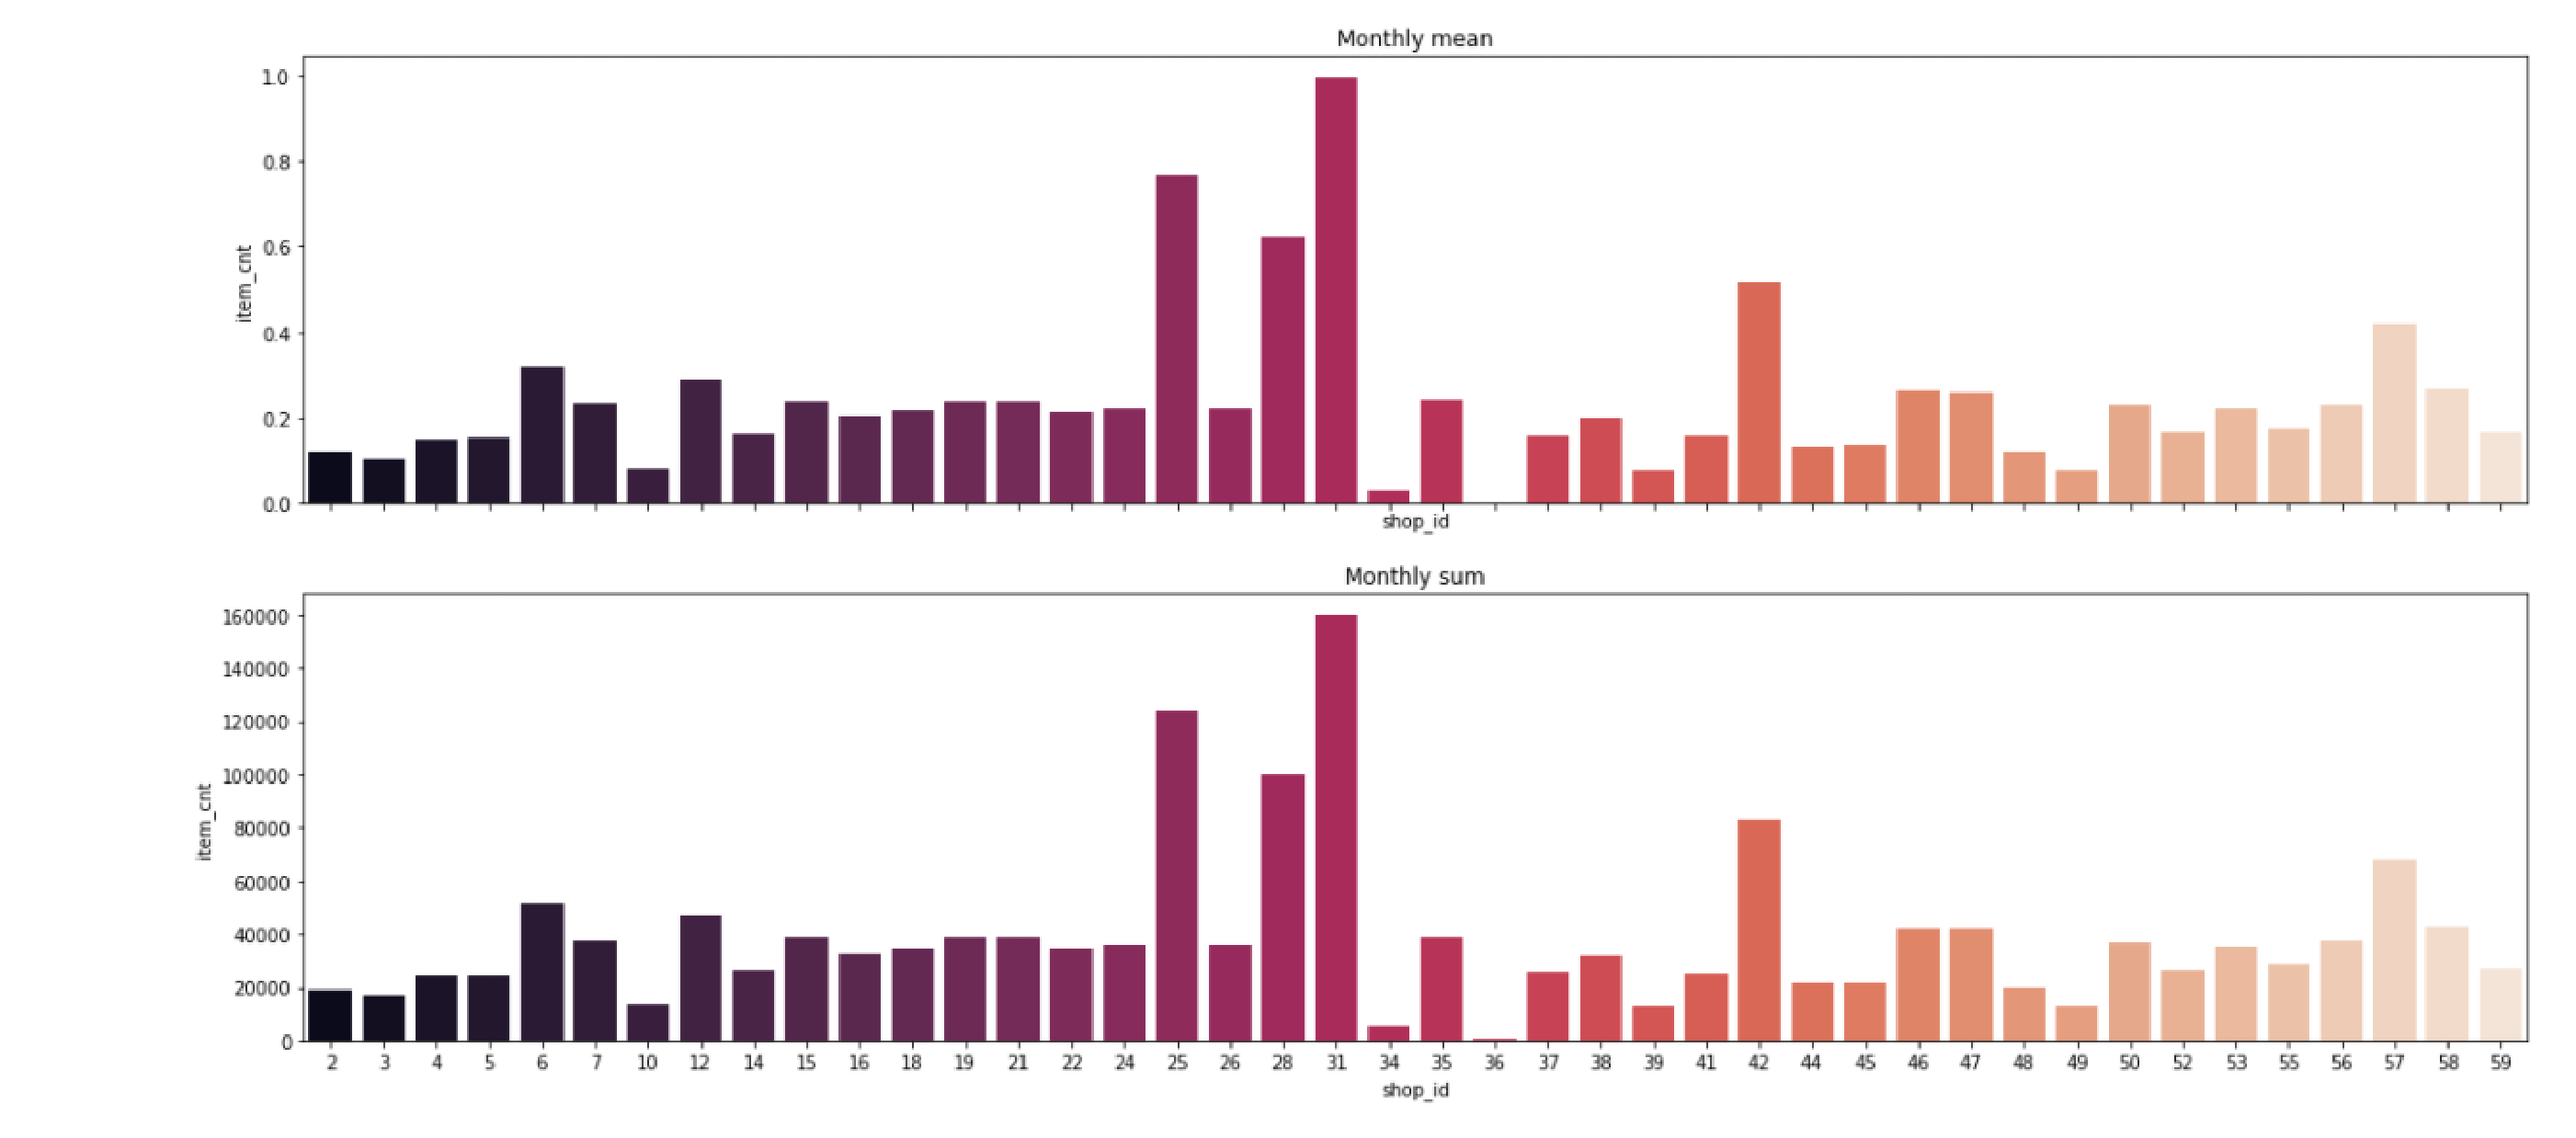
\includegraphics[scale=0.4]{picture/data_30.eps}
  \end{figure}
  \begin{center}
    \textbf{Figure 2}~~shop_count.\\
  \end{center}
\end{slide}
%%
%%==========================================================================================

%%==========================================================================================
%%
\begin{slide}[toc=,bm=]{Sales of different category}
  \begin{figure}
    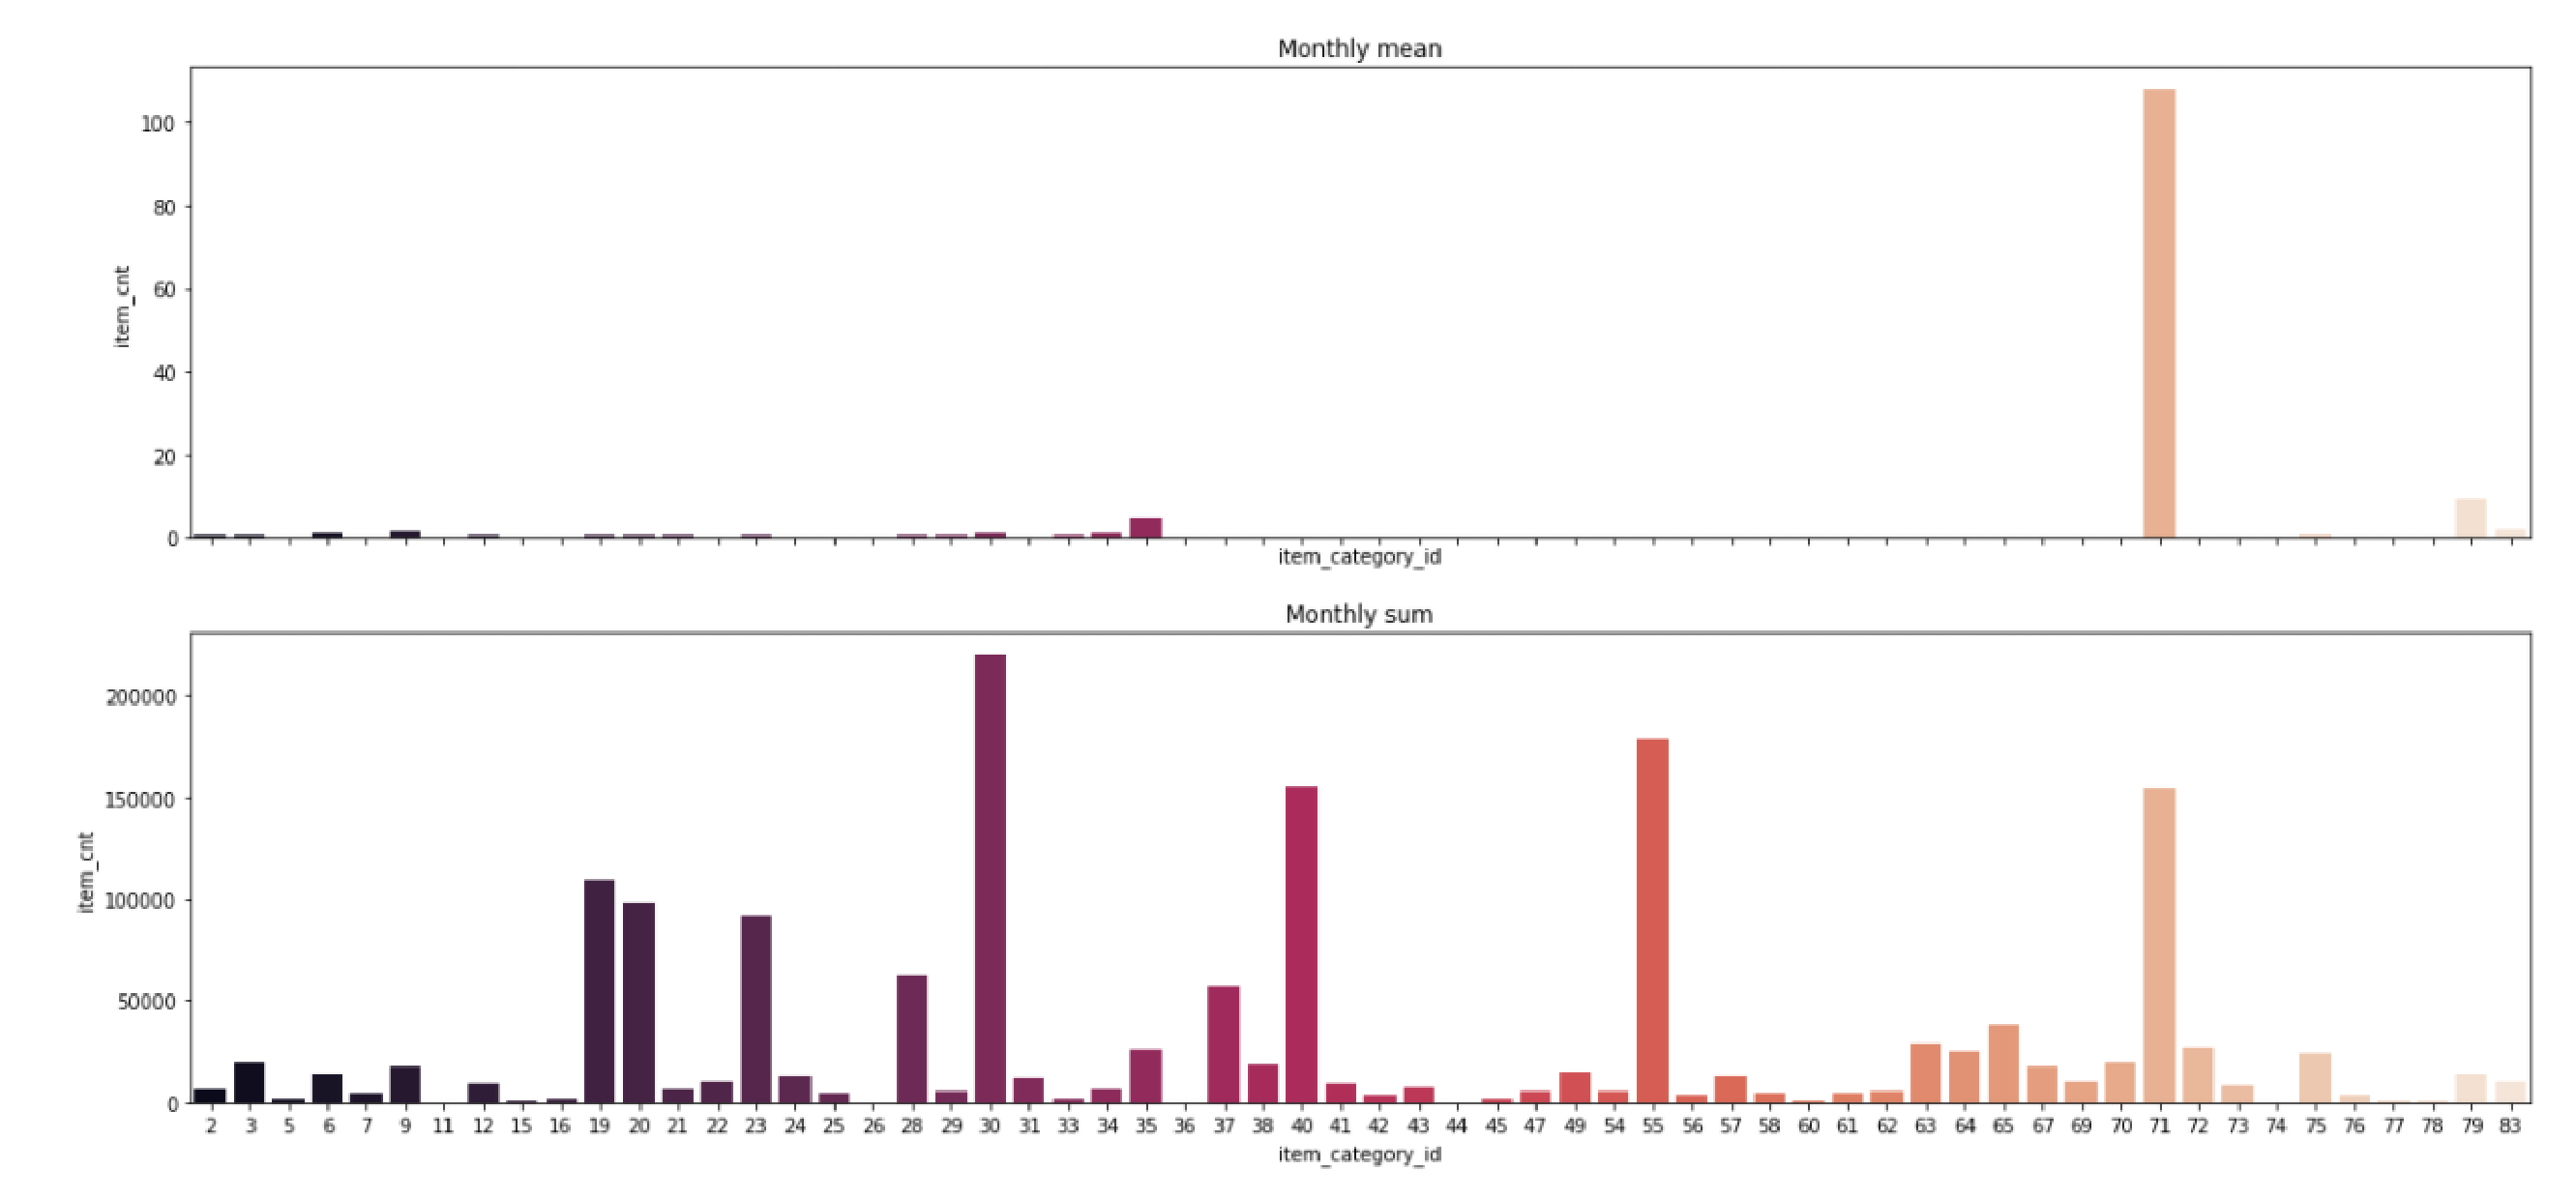
\includegraphics[scale=0.4]{picture/data_31.eps}
  \end{figure}
  \begin{center}
    \textbf{Figure 3}~~item_category_count.\\
  \end{center}
\end{slide}
%%
%%==========================================================================================


%%==========================================================================================
%%
\begin{slide}[toc=,bm=]{Item and Shop Information}
  \twotonebox{\parbox{.1\textwidth}{categories of items}}{\parbox{.76\textwidth}
  {
    large categories, small categories, we separate them, and code them separately to facilitate subsequent feature extraction
  }}
  \twotonebox{\parbox{.1\textwidth}{Shop information}}{\parbox{.76\textwidth}
  {
    the city where the store is located, the type of store, which we separate and encode separately for subsequent feature extraction
  }}
\end{slide}
%%
%%==========================================================================================

\section{Model}

%%==========================================================================================
%%
\begin{slide}[toc=,bm=]{decision tree}
  \twotonebox{\parbox{.1\textwidth}{Dicision tree}}{\parbox{.76\textwidth}
  {
    In machine learning, decision tree is a prediction model, which represents a mapping relationship between object attributes and object values. Each node in the tree represents an object, and each branch path represents a possible attribute value, while each leaf node corresponds to the value of the object represented by the path from the root node to the leaf node. The decision tree has only a single output, if you want to have complex output, you can establish an independent decision tree to deal with different outputs. Decision tree is a frequently used technology in data mining, which can be used to analyze data, and also can be used for prediction.
  }}
\end{slide}
%%
%%==========================================================================================


%%==========================================================================================
%%
\begin{slide}[toc=,bm=]{Model selection}
  \begin{itemize}
    \item GBDT
    \item Xgboost
    \item lightgbm
    \item neural network
  \end{itemize}
\end{slide}
%%
%%==========================================================================================


%%==========================================================================================
%%
\begin{slide}[toc=,bm=]{Method One}
  \twotonebox{\parbox{.1\textwidth}{Method}}{\parbox{.76\textwidth}
  {
    The sales of the 34th month are regarded as the sales of the 35th month
  }}
  \twotonebox{\parbox{.1\textwidth}{operation}}{\parbox{.76\textwidth}
  {
    Count the sales volume of each item in each store in the 33rd month and merge it with test
  }}
  \twotonebox{\parbox{.1\textwidth}{Result}}{\parbox{.76\textwidth}
  {
    RMSE=1.16777
  }}
\end{slide}
%%
%%==========================================================================================

%%==========================================================================================
%%
\begin{slide}[toc=,bm=]{Method Two}
  \twotonebox{\parbox{.1\textwidth}{Data feature}}{\parbox{.76\textwidth}
  {
    'date_block_num', 'shop_id', 'item_id', 'item_category_id', 'cat_type_code', 'cat_subtype_code', 'shop_city_code', 'shop_type_code'
  }}
  \twotonebox{\parbox{.1\textwidth}{Monthly sales feature}}{\parbox{.76\textwidth}
  {
    \begin{itemize}
      \item item_cnt_month
      \item date_avg_item_cnt
      \item date_item_avg_item_cnt
      \item date_shop_avg_item_cnt
      \item date_cat_avg_item_cnt
      \item date_cat_shop_avg_item_cnt
      \item date_type_avg_item_cnt
      \item date_item_type_avg_item_cnt
      \item date_city_avg_item_cnt
   \end{itemize}
  }}
  \twotonebox{\parbox{.1\textwidth}{Historical feature}}{\parbox{.76\textwidth}
  {
    delay:1,2,3,6,12
  }}
\end{slide}
%%
%%==========================================================================================

%%==========================================================================================
%%
\begin{slide}[toc=,bm=]{Method Two}
  \begin{figure}
    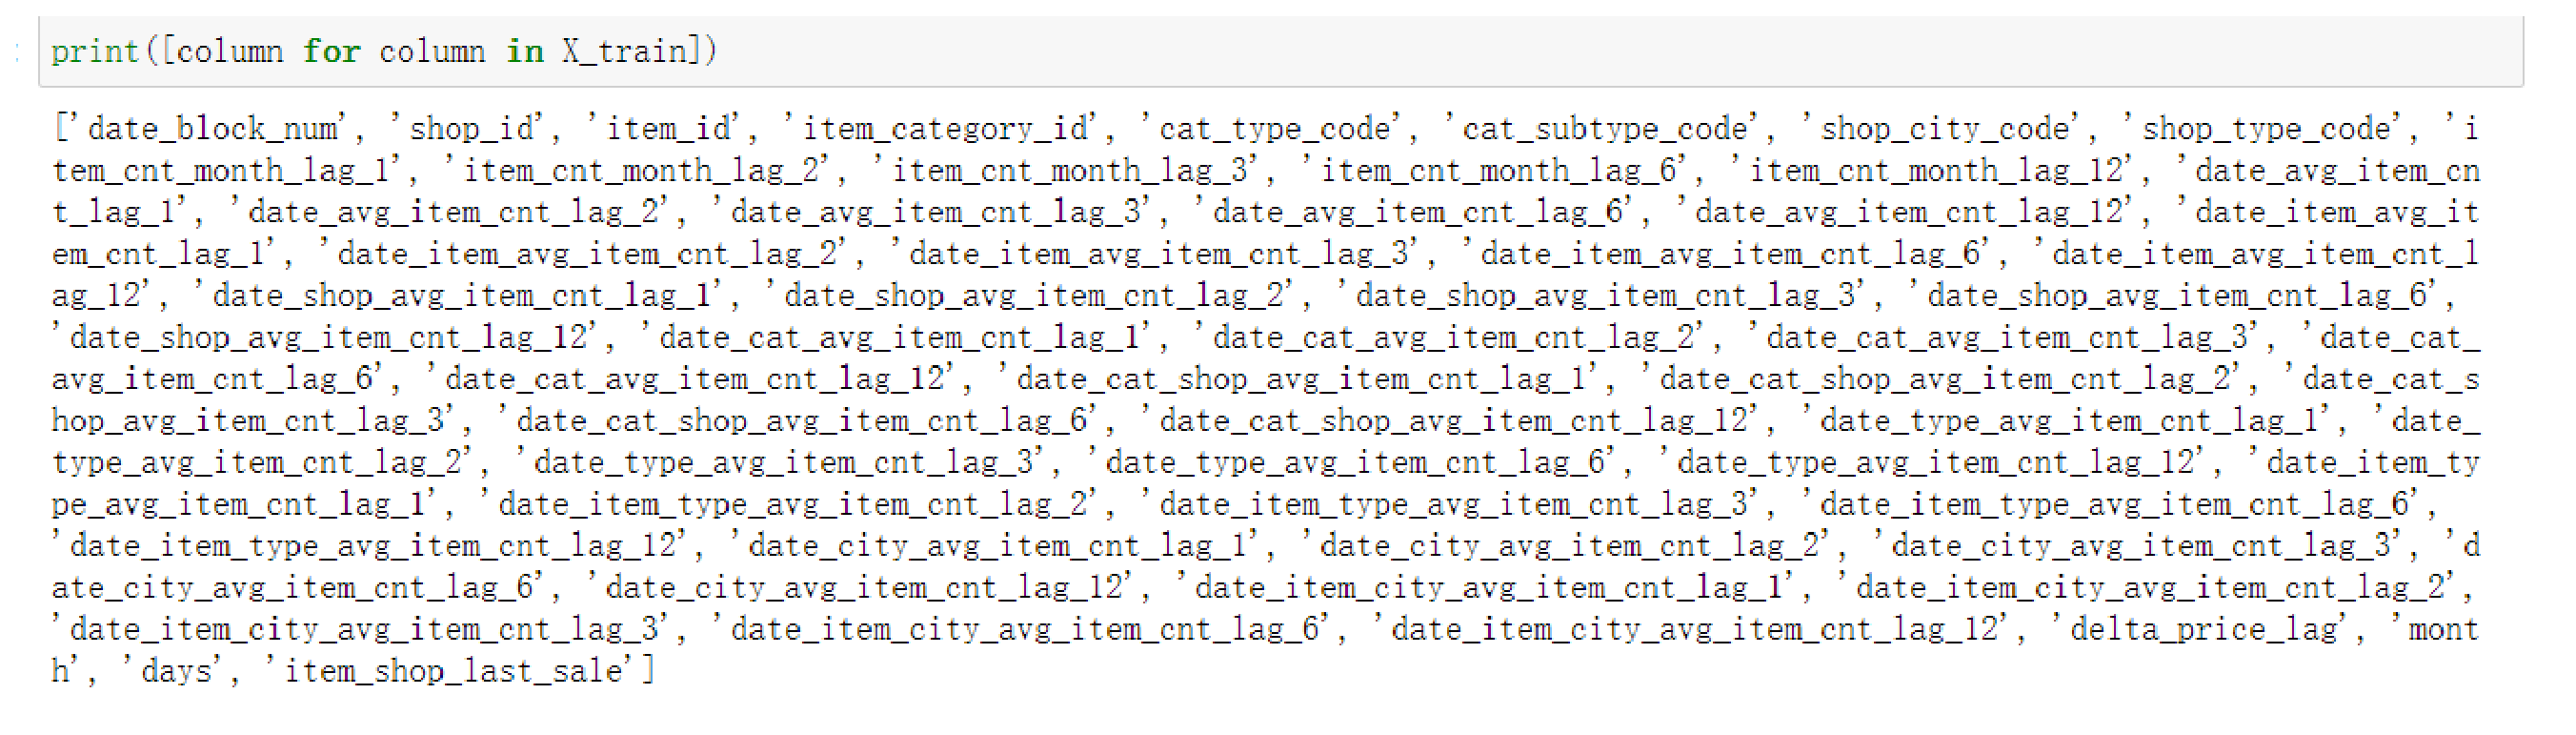
\includegraphics[scale=0.4]{picture/data_16.eps}
  \end{figure}
\end{slide}
%%
%%==========================================================================================

%%==========================================================================================
%%
\begin{slide}[toc=,bm=]{Method Two}
  \twotonebox{\parbox{.1\textwidth}{Result}}{\parbox{.76\textwidth}
  {\begin{itemize}
    \item valid_1's rmse: 0.880256
  \end{itemize}
  }}
\end{slide}
%%
%%==========================================================================================


\end{document}
